%\graphicspath{{/Users/emiliendurif/Documents/prepa/sujets/DS/flir/images/}}
%\vspace{-1.5cm}
\begin{huge}
\textbf{Vision en réalité augmentée pour hélicoptère}
\end{huge}

\section*{Présentation du système}

\subsection*{Contexte}
\begin{figure}[h]
\begin{center}
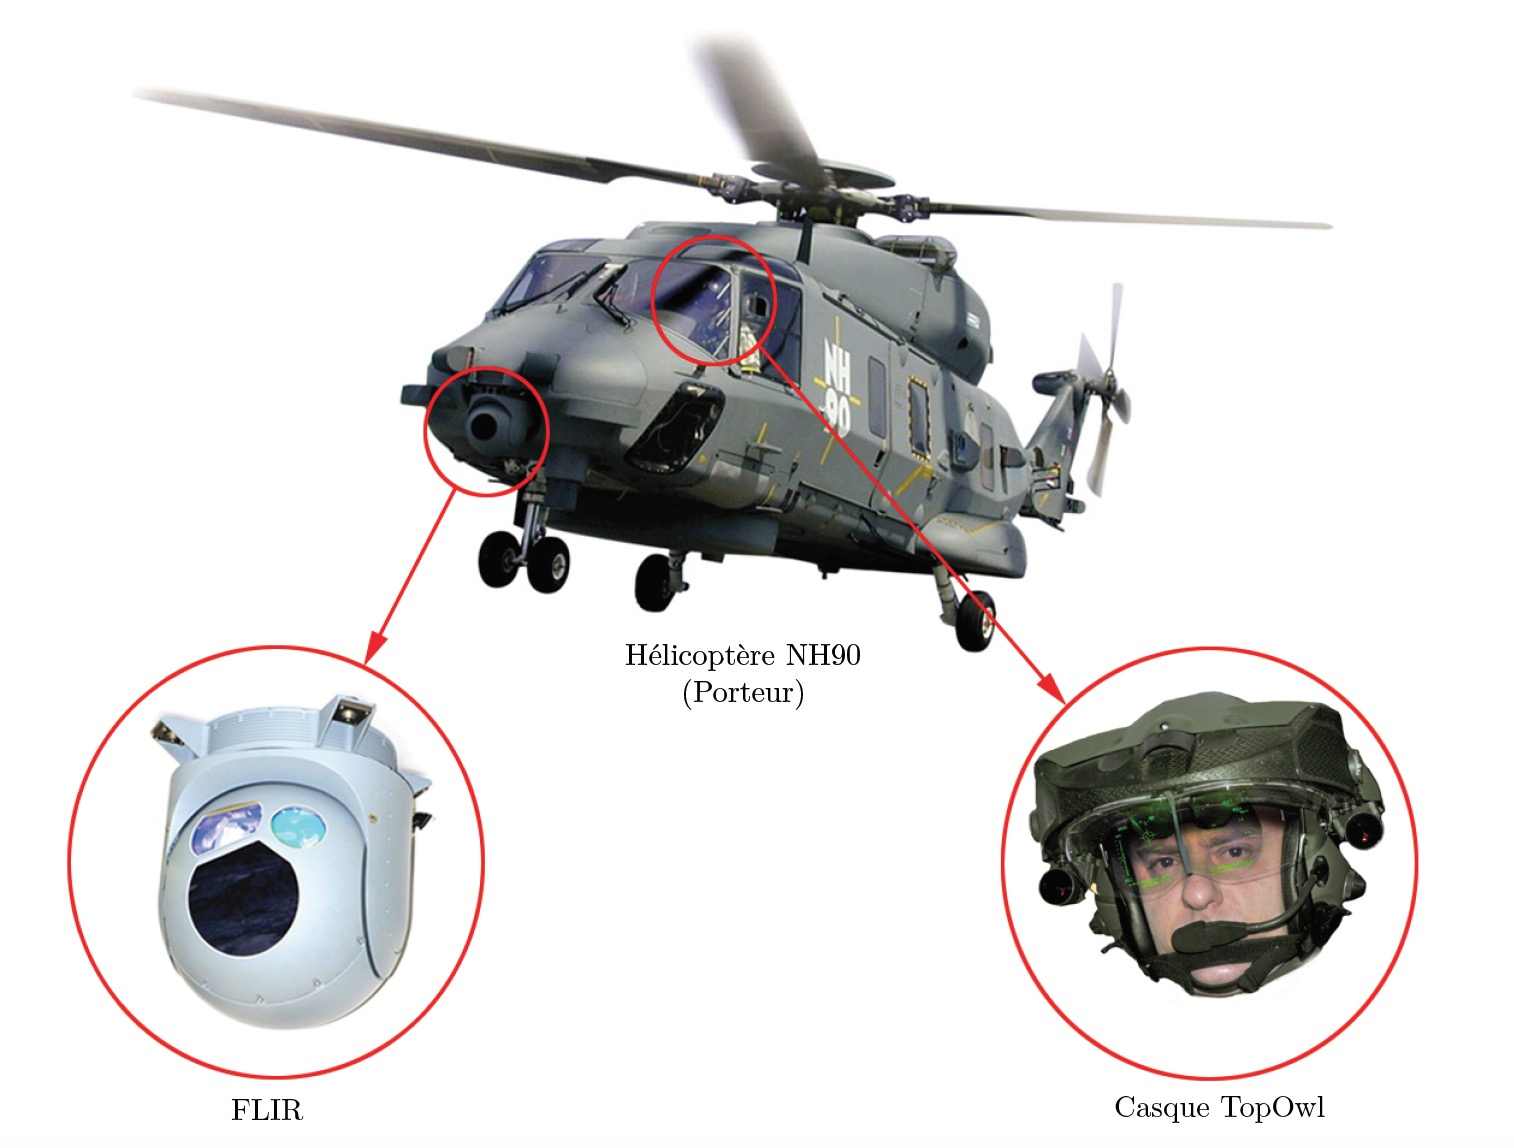
\includegraphics[width=0.6\textwidth]{figure1.jpg}
\caption{Hélicoptère NH90 équipé du système de vision en réalité augmentée\label{fig1}}
\end{center}
\end{figure}

Les hélicoptères sont des aéronefs dont l'un des intérêts est de pouvoir effectuer des vols proches du relief. Suivant les conditions climatiques (tempête de sable, brouillard ou vol de nuit par exemple), la propre vision du pilote et l'instrumentation de navigation classique peuvent être insuffisantes pour assurer la sécurité du vol. Pour pallier cela, la société Thalès propose un système de vision en réalité augmentée composée du casque TopOwl et d'un FLIR (\textit{Forward Looking InfraRed}).

\begin{figure}[h]
\centering
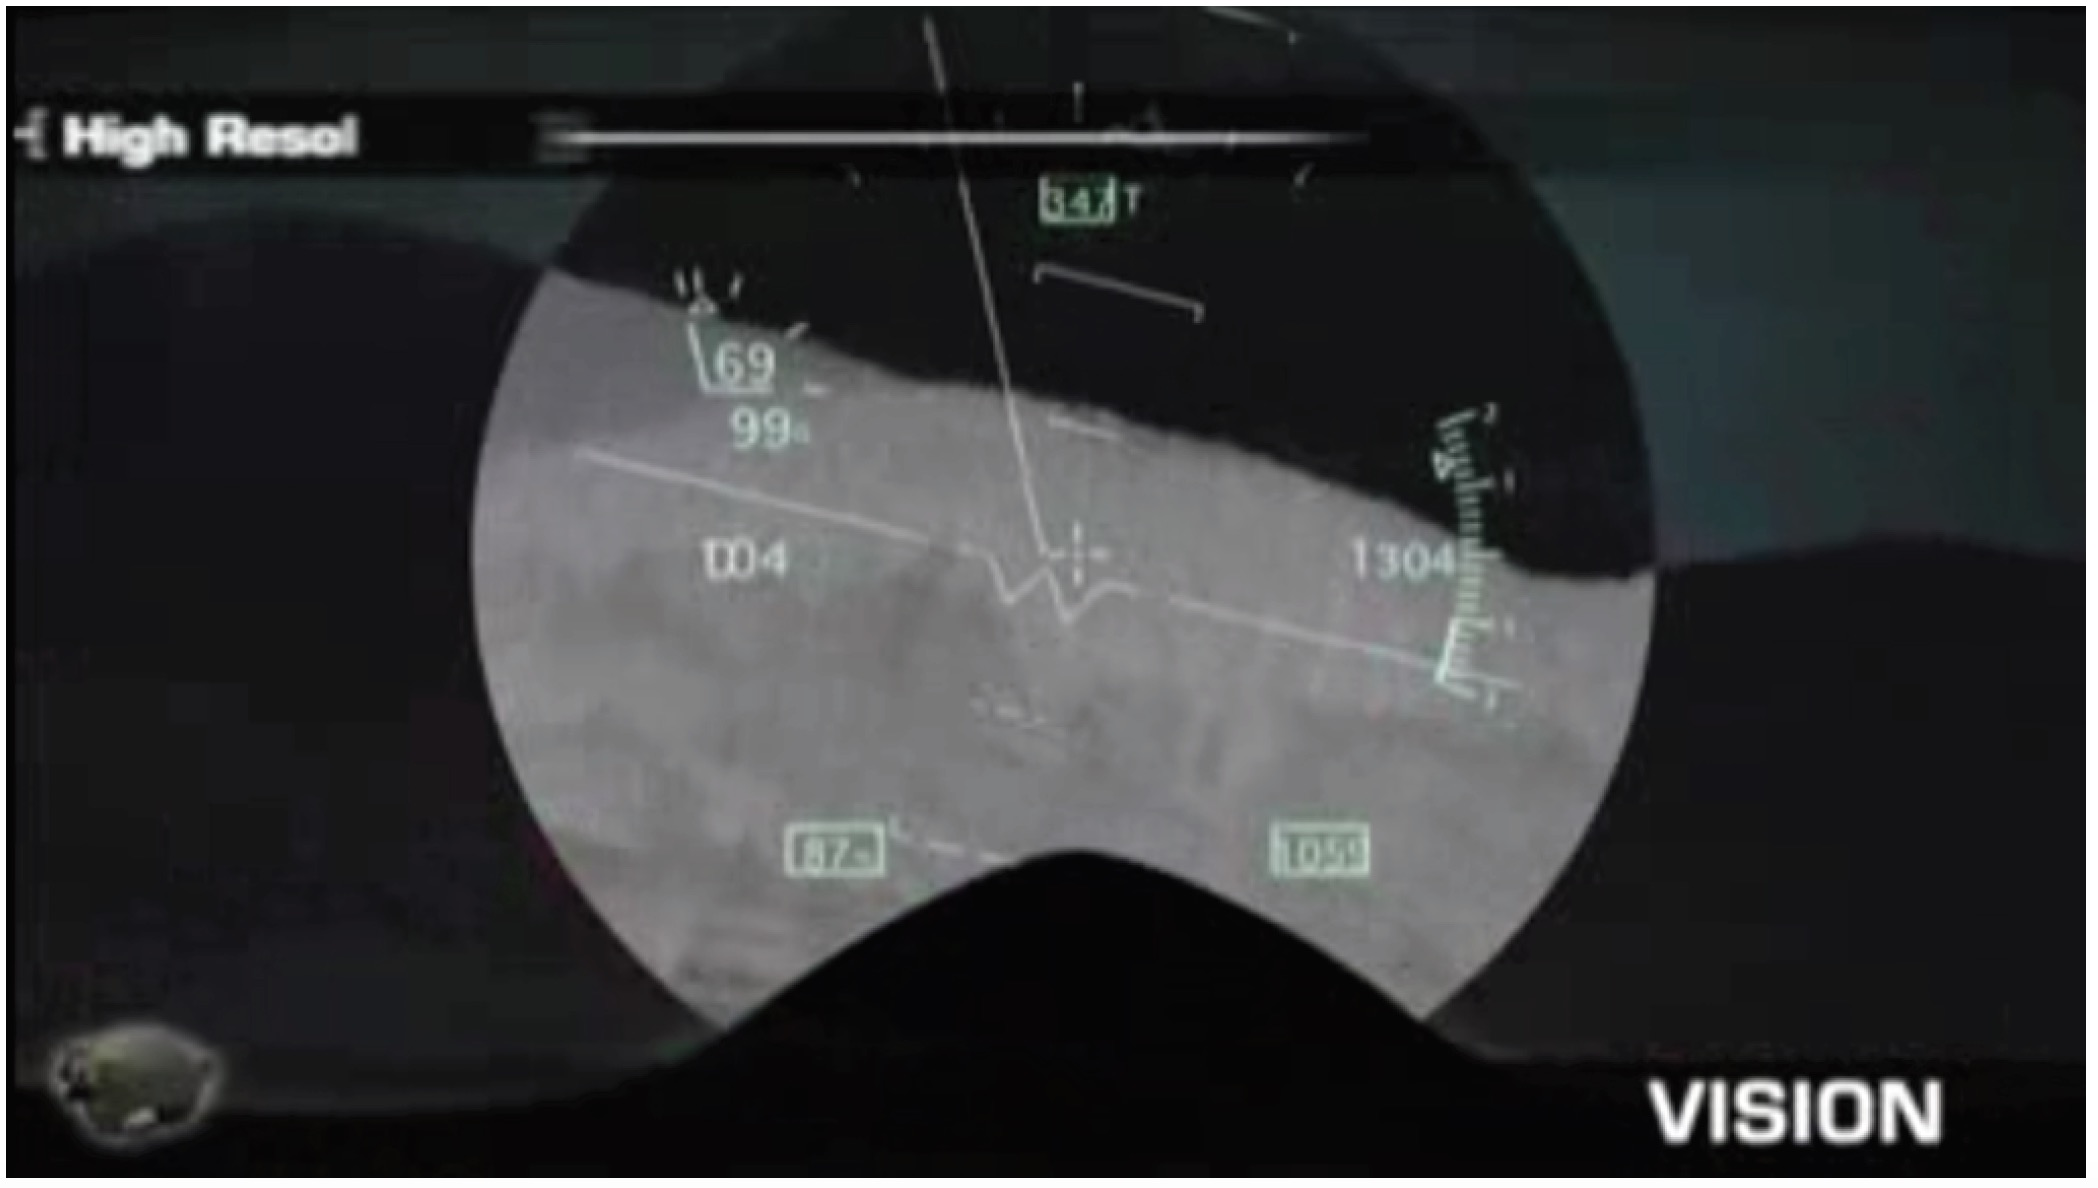
\includegraphics[width=0.8\textwidth]{figure2.jpg}
\caption{Hélicoptère NH90 équipé du système de vision en réalité augmentée\label{fig2}}
\end{figure}

%\FloatBarrier
La vision en réalité augmentée consiste à venir projeter
sur la visière du casque TopOwl une image prise par une
des caméras du \textbf{FLIR}. L'image projetée se superpose au
paysage visible à travers la visière de façon à améliorer
la vision du pilote. De nuit, par temps de brouillard ou
de tempête, l'image peut être une image infra-rouge ou
thermique. En plus de l'image, des informations peuvent être ajoutées sur la projection ; par exemple des données
GPS, des routes, des informations de vol.

Le FLIR est une boule optronique modulaire pouvant intégrer plusieurs capteurs différents dont une caméra
thermique, une caméra couleur TV HD, ainsi qu'une caméra très bas niveau de lumière. Cet ensemble est
orientable et gyrostabilisé, c'est-à-dire en particulier que les caméras sont capables de garder une même ligne
de visée par rapport au référentiel terrestre, quels que soient les mouvements de l'hélicoptère NH90 qui sera
appelé \textbf{porteur} dans la suite du sujet. Le casque TopOwl est placé sur la tête du pilote et le \textbf{FLIR} sur l'avant
du porteur.
Une étude relative à la physique du casque TopOwl a permis de déterminer certaines de ses performances qui
seront données au moment opportun. Ce sujet a pour objet l'étude des performances du sous-système FLIR,
intégré dans le système de vision en réalité augmentée. La problématique globale est de vérifier que l'image
projetée sur la visière du casque TopOwl est utilisable par le pilote, c'est-à-dire :
\begin{itemize}
\item  que la ligne de visée des caméras est conforme à la ligne de visée du pilote (les lignes de visée sont définies
par rapport au référentiel terrestre) ;
\item que le retard entre la prise de vue et son affichage n'est pas visible par le pilote (retard inférieur à la
persistance rétinienne) ;
\item que la prise de vue n'est pas perturbée par les mouvements du porteur.
\end{itemize}


\subsection*{Exigences}

\begin{figure}[!htb]
\begin{center}
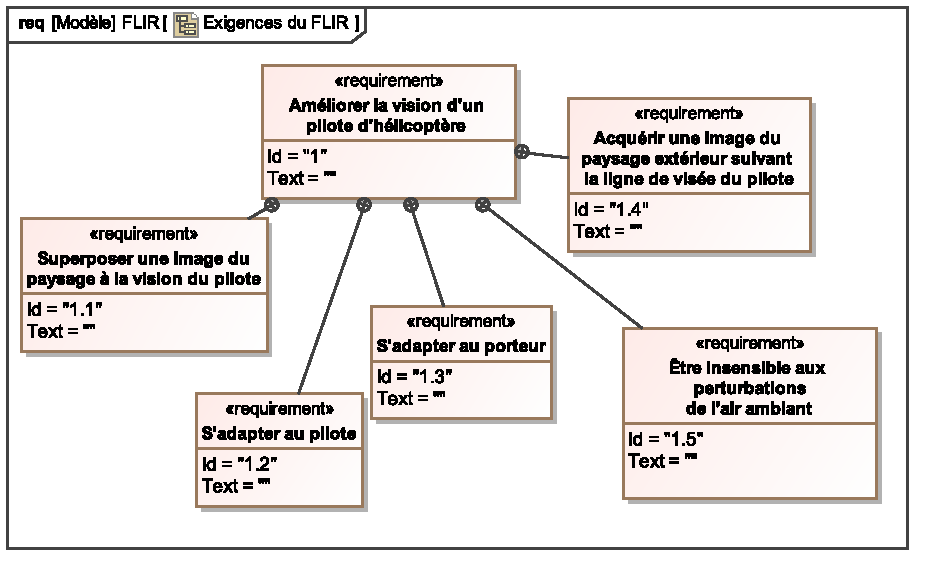
\includegraphics[width=0.7\textwidth]{req_flir.pdf}
\caption{Diagramme des exigences partiel \label{req_flir}}
\end{center}
\end{figure}


\begin{table}[!htb]
\begin{center}
\begin{tabular}{|p{0.3\textwidth}|p{0.3\textwidth}|p{0.3\textwidth}|}
\hline 
\textbf{Exigence} & \textbf{Critère} & \textbf{Valeur} \\ 
\hline 
1.1 Superposer une image du paysage à la vision du pilote & Résolution (largeur du plus petit
objet visible sur l'image) & 1 m pour un objet situé à 1 km de
distance du pilote \\ 
\cline{2-3} 
& Précision (décalage entre l'image
projetée sur la visière du TopOwl et
le paysage réel) & Erreur de superposition inférieure
ou égale à 1 pixel\\ 
\cline{2-3}  
 & Latence d'affichage (temps entre la
prise de vue et son affichage sur la
visière du TopOwl) & Inférieure ou égale à la persistance
rétinienne ($t_{ret} \leq 120 ms$) \\ 
\cline{2-3}  
 & Stabilité de l'image projetée sur la
visière & Oscillations d'amplitude inférieure
à 1/2 pixel \\ 
\hline
\end{tabular} 
\caption{Cahier des charges partiel du système de vision en réalité augmentée \label{tab1}}
\end{center}
\end{table}

L'étude se décompose en trois parties. Une étude de la physique du casque TopOwl ayant été effectuée dans
le sujet de physique, la partie 2 porte sur la détermination des performances (rapidité et précision) à atteindre
par le sous-système FLIR en fonction du cahier des charges du système de vision en réalité augmentée et
des performances des autres sous-systèmes. L'objectif des parties 3 et 4 est d'analyser le choix d'architecture du
FLIR en vue de valider les hypothèses simplificatrices concernant son comportement. La partie 5 consiste à
vérifier si les solutions retenues, tant au niveau de l'architecture que de la commande, permettent d'atteindre
les performances attendues du FLIR
